% !TEX root = Experiment41.tex

 
 \chapter{The Standard Model of Particle Physics}
 
 
 
After closer investigation of cosmic radiation, many new particles were discovered, such as neutral Kaons \PKzero in 1947. As new techniques, such as particle accelerators were improved, this `Particle Zoo' became more and more confusing to physicists. In the 1960s and 70s, a new model emerged: the Standard Model which brought order to the apparent chaos. It did so by articulating the phenomenology of known fundamental interactions into a single self-consistent, locally gauge-invariant quantum field theory centered around electromagnetism (Quantum Electro-Dynamics or \textit{QED}), the strong nuclear force (Quantum Chromo-Dynamics or \textit{QCD}) and the weak nuclear force.

Those interactions are mediated by spin-1 particles, the so called \textit{vector-bosons}: the photon \Pgamma mediates QED, eight massless but coloured gluons \Pgluon mediate QCD and three massive bosons \PZ, \PWpm mediate the weak interaction. Finally a single spinless massive \textit{scalar boson}, the so called \textit{Higgs Boson} was observed in 2012 and allows for massive bosons and at least certain fermions to be massive. All those bosons can be found in Table \ref{tab:bosons}. Each interaction takes place via the exchange of its bosons, for example, the $\beta^{-}$-decay of $^{137}\text{Cs}$ to $^{137}\text{Ba}$ can in fact be seen as a neutron's \Pdown emitting a \PWminus and thus becoming a \Pup, causing the neutron to become a proton. This reaction can be seen in Figure \ref{fig:betadecay}.
Matter however is made of fermions, particle with spin $\frac{1}{2}$, those, in the Standard Model are classified as \textit{quarks} and \textit{leptons}.
The Standard Model was observed to hold  6 massive quarks, reacting to all three interactions, 3 charged leptons, sensitive to electromagnetism and the weak interaction, and 3 neutral leptons, \textit{neutrinos}, which only interact through the weak interaction. They can be found in Table \ref{tab:SM}.

\begin{table}[htbp]
\centering
\resizebox{\linewidth}{!}{%
\begin{tabular}{|c|c|c|c|c|c|c|}
\hline
\textbf{Generation} & \multicolumn{2}{c|}{\textbf{1}} & \multicolumn{2}{c|}{\textbf{2}} & \multicolumn{2}{c|}{\textbf{3}} \\ \hline
& Fermion & Mass [MeV] & Fermion & Mass [MeV] & Fermion & Mass [MeV] \\ \hline
Up-type quarks ($q=\frac{2}{3}$) & up (\Pup) & $\sim 2.2$ & charm (\Pcharm) & $\sim 1300$ & top (\Ptop) & $173000 $  \\ \hline
Down-type quarks ($q=\frac{+2}{3}$) & down (\Pdown) & $\sim 4.7$ & strange (\Pstrange) & $\sim 95$ & beauty/bottom (\Pbottom) & $\sim 4200$ \\ \hline
Charged leptons ($q=\frac{-1}{2}$) & electron (\Pelectron) & $0.511$  & muon (\Pmuon) & $113$ & tau (\Ptauon) & $1780$  \\ \hline
Neutrinos ($q=0$) &  electron neutrino (\Pnue) & $\sim 0$ & muon neutrino (\Pnum) & $\sim 0$ & tau neutrino (\Pnut) & 0 \\ \hline
\end{tabular}}
\caption{Standard Model fermions.}
\label{tab:SM}
\end{table}

\begin{table}[htbp]
\centering
\scriptsize
\setlength\tabcolsep{2pt}
\begin{tabular}{|c|c|c|c|c|c|c|c|}
\hline
\textbf{Interaction} & \textbf{Boson} & \textbf{Mass [GeV]} & \textbf{Range [m]} & \textbf{Time scale [s]} & \textbf{spin} & \textbf{coupling} & \textbf{Fields} \\ \hline
Strong & gluon (\Pgluon)& 0 & $10^{-15}$ & $10^{-23}$ & 1 & $\sim 1$ & Quarks \\ \hline
Electromagnetic & photon (\Pgamma) & 0 & $\inf$ & $10^{-20}$ & 1 & $1/137$ & Electric charge \\ \hline
Weak & Z-zero boson (\PZzero), W bosons (\PWpm) & 91.2, 80.4 &  $\sim 10^{-17}$ & $10^{-8}$ & 1 & $10^{-5}$ & Quarks and leptons \\ \hline
Higgs & boson \PHiggs & $ 125.2$ & $\sim 10^{-18}$ &  $\sim 10^{-22}$ & 0 & variable & Massive fields \\ \hline
Gravity & graviton ($g$) & 0 & $\inf$ & - & 2 & $> 10^{-41}$ & Massive fields \\ \hline

\end{tabular}
\caption{Standard Model force carriers.}
\label{tab:bosons}
\end{table}


\begin{figure}[htbp]
\centering
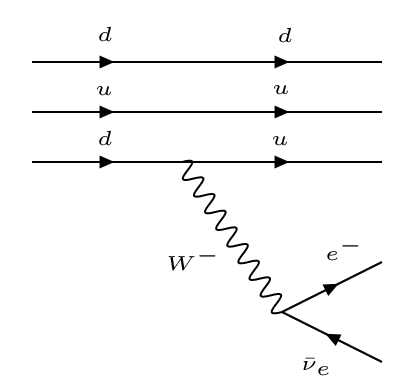
\includegraphics[width=0.5\linewidth]{./fig/betadecay.png}
\caption{Weak decay of a neutron to a proton.}
\label{fig:betadecay}
\end{figure}

Ordinary matter is overwhelmingly composed of first generation particles: \textit{up} and \textit{down}- type quarks and \textit{electrons}, a proton is notably composed of two up-type quarks and one down-type quark while a neutron is composed of a single up-type quark and two down-type quarks. It should be noticed that this is mostly due to the unstable nature of particles from Generation 2 and 3 (with the notable exception of neutrinos). Those particles will decay into lighter ones, it should be noted that, as a general rule, heavier particles decay faster and thus have a shorter lifetime. 

